\documentclass[11pt]{article}
\usepackage[margin=1in]{geometry}
\usepackage{amsmath,amssymb,bm}
\usepackage{graphicx}
\usepackage{booktabs}
\usepackage{placeins}
\usepackage{float}
\usepackage{enumitem}
\usepackage[hidelinks]{hyperref}
\setlength{\parskip}{4pt}
\renewcommand{\topfraction}{0.9}
\renewcommand{\bottomfraction}{0.8}
\renewcommand{\textfraction}{0.07}
\renewcommand{\floatpagefraction}{0.85}
\setcounter{topnumber}{3}\setcounter{totalnumber}{4}
\setlength{\parindent}{0pt}

\title{CSc 8830 Computer Vision, Module 4, Question 3\\[4pt]
\large Edge Detection and Region Segmentation in the Fourier Domain}
\author{Liberty Ikpeogu}
\date{}

\begin{document}
\maketitle

\section{Setup: the 2D Fourier transform}

For a continuous image $f(x,y)$ the Fourier transform and its inverse are
\begin{align}
F(u,v) &= \iint_{-\infty}^{\infty} f(x,y)\, e^{-j2\pi(ux+vy)}\,dx\,dy, \label{eq:ft}\\
f(x,y) &= \iint_{-\infty}^{\infty} F(u,v)\, e^{\,j2\pi(ux+vy)}\,du\,dv, \label{eq:ift}
\end{align}
with $(u,v)$ in cycles per unit length. For an $M\times N$ digital image, the discrete Fourier transform (DFT) is
\begin{equation}
F(u,v)=\sum_{x=0}^{M-1}\sum_{y=0}^{N-1} f(x,y)\,e^{-j2\pi\left(\frac{ux}{M}+\frac{vy}{N}\right)},
\qquad u=0,\dots,M-1,\; v=0,\dots,N-1 .
\end{equation}
We write $\rho=\sqrt{u^2+v^2}$ for radial frequency.

\paragraph{Convolution theorem.} Every result below rests on this identity. For $g=h*f$,
\[
G(u,v)=\iint\!\!\iint h(s,t)\,f(x-s,y-t)\,e^{-j2\pi(ux+vy)}\,ds\,dt\,dx\,dy .
\]
Substituting $x'=x-s,\ y'=y-t$ splits the exponential into $e^{-j2\pi(us+vt)}e^{-j2\pi(ux'+vy')}$, and the integral factors:
\begin{equation}
\boxed{\,g=h*f \;\Longleftrightarrow\; G(u,v)=H(u,v)\,F(u,v)\,} \label{eq:conv}
\end{equation}
Any linear, shift-invariant filter therefore acts in the frequency domain as a pointwise multiplication by its transfer function $H(u,v)$. Designing an edge detector reduces to choosing $H$.

\section{Why edges live at high frequencies}

\subsection{The derivative theorem}
Differentiate the inverse transform \eqref{eq:ift} with respect to $x$. Only the exponential depends on $x$:
\[
\frac{\partial f}{\partial x}=\iint F(u,v)\,\frac{\partial}{\partial x}e^{\,j2\pi(ux+vy)}\,du\,dv
=\iint \big[\,j2\pi u\,F(u,v)\big]\,e^{\,j2\pi(ux+vy)}\,du\,dv .
\]
The bracket is, by definition, the transform of $\partial f/\partial x$. Repeating for $y$:
\begin{equation}
\mathcal{F}\!\left\{\frac{\partial f}{\partial x}\right\}=j2\pi u\,F(u,v),\qquad
\mathcal{F}\!\left\{\frac{\partial f}{\partial y}\right\}=j2\pi v\,F(u,v). \label{eq:deriv}
\end{equation}
The gradient filters $H_x=j2\pi u$ and $H_y=j2\pi v$ have magnitude growing linearly with frequency: they suppress slowly varying content and amplify rapid change. Differentiation is high-pass filtering.

\subsection{The spectrum of an edge}
Model a vertical step edge of contrast $A$ at $x_0$ as $f(x)=A\,\mathcal{H}(x-x_0)$, where $\mathcal{H}$ is the unit step. Using $\mathcal{F}\{\mathcal{H}(x)\}=\frac{1}{j2\pi u}+\frac12\delta(u)$ and the shift theorem,
\begin{equation}
F(u)=A\,e^{-j2\pi u x_0}\left[\frac{1}{j2\pi u}+\tfrac12\delta(u)\right],
\qquad |F(u)|=\frac{A}{2\pi|u|}\ \text{ for } u\neq 0 . \label{eq:step}
\end{equation}
A step spreads energy over all frequencies with a slow $1/|u|$ decay, far slower than the rapid falloff of a smooth region. Applying \eqref{eq:deriv}:
\[
\mathcal{F}\{f'(x)\}=j2\pi u\cdot\frac{A\,e^{-j2\pi u x_0}}{j2\pi u}=A\,e^{-j2\pi u x_0}
\;\Longleftrightarrow\; f'(x)=A\,\delta(x-x_0).
\]
The derivative flattens the spectrum to constant magnitude $A$, and the inverse transform concentrates all of it at $x_0$: a spike at the edge whose height encodes the contrast. The linear phase $e^{-j2\pi u x_0}$ carries the edge location.

\subsection{\texorpdfstring{Finite differences are approximations of $j2\pi u$}{Finite differences approximate j2 pi u}}
The central difference $d(x)=\tfrac12[f(x+1)-f(x-1)]$ has transfer function
\[
H_{\text{cd}}(u)=\tfrac12\left(e^{j2\pi u}-e^{-j2\pi u}\right)=j\sin(2\pi u)\approx j2\pi u\quad\text{for small }u .
\]
The Sobel operator multiplies this by a $[1\ 2\ 1]/4$ smoother along the other axis, whose transform is $\tfrac14(2+2\cos 2\pi v)=\cos^2(\pi v)$, so
\begin{equation}
H_{\text{Sobel},x}(u,v)\propto j\sin(2\pi u)\cos^2(\pi v).
\end{equation}
Sobel is a derivative along $u$ combined with a low-pass along $v$. The frequency view explains its noise resistance directly.

\subsection{The Laplacian}
Applying \eqref{eq:deriv} twice in each direction and summing:
\begin{equation}
\mathcal{F}\{\nabla^2 f\}=\left[(j2\pi u)^2+(j2\pi v)^2\right]F=-4\pi^2(u^2+v^2)\,F=-4\pi^2\rho^2F. \label{eq:lap}
\end{equation}
The Laplacian is isotropic (it depends on $\rho$ alone) and grows quadratically, so it is an even stronger high-pass. The discrete 5-point stencil gives $H=2\cos2\pi u+2\cos2\pi v-4=-4(\sin^2\pi u+\sin^2\pi v)$, which matches $-4\pi^2\rho^2$ near the origin.

\section{Noise, and why edge detectors need a band-pass}

Write the observed image as $f=s+n$ with white noise $n$ of power spectral density $\sigma_n^2$ (flat in frequency). After a filter $H$, the output noise power is
\begin{equation}
P_n=\sigma_n^2\iint |H(u,v)|^2\,du\,dv .
\end{equation}
For the gradient, $|H|^2=4\pi^2\rho^2$. In polar coordinates up to a band limit $\rho_{\max}$,
\[
P_n=\sigma_n^2\int_0^{2\pi}\!\!\int_0^{\rho_{\max}}4\pi^2\rho^2\,\rho\,d\rho\,d\theta=2\pi^3\sigma_n^2\rho_{\max}^4 .
\]
Noise power grows as $\rho_{\max}^4$ (and as $\rho_{\max}^6$ for the Laplacian) while the edge signal in \eqref{eq:step} decays as $1/\rho$. At high frequencies noise wins, so a practical detector must cap the gain at high $\rho$. The standard choice is a Gaussian low-pass:
\begin{equation}
g_\sigma(x,y)=\frac{1}{2\pi\sigma^2}e^{-\frac{x^2+y^2}{2\sigma^2}}
\;\Longleftrightarrow\;
G_\sigma(u,v)=e^{-2\pi^2\sigma^2(u^2+v^2)} . \label{eq:gauss}
\end{equation}
A Gaussian transforms to a Gaussian, with widths inversely related ($\sigma$ in space, $1/(2\pi\sigma)$ in frequency).

\subsection{Laplacian of Gaussian (LoG) as a band-pass filter}
Smoothing then differentiating equals differentiating the kernel, $\nabla^2(g_\sigma*f)=(\nabla^2 g_\sigma)*f$. Combining \eqref{eq:lap} and \eqref{eq:gauss}:
\begin{equation}
H_{\text{LoG}}(\rho)=-4\pi^2\rho^2\,e^{-2\pi^2\sigma^2\rho^2}. \label{eq:log}
\end{equation}
This is zero at $\rho=0$ (it ignores uniform brightness) and decays to zero at high $\rho$ (it rejects noise). The peak response comes from
\[
\frac{d}{d\rho}\left(\rho^2e^{-a\rho^2}\right)=2\rho\,e^{-a\rho^2}(1-a\rho^2)=0,\quad a=2\pi^2\sigma^2
\;\Longrightarrow\;
\boxed{\rho^*=\frac{1}{\sqrt{2}\,\pi\sigma}}
\]
so $\sigma$ selects the scale of edge the detector responds to most. For $\sigma=2$ px, $\rho^*\approx0.113$ cycles/px (Figure~\ref{fig:filters}). The difference of two Gaussians, $G_{\sigma_1}-G_{\sigma_2}$, approximates the same band-pass shape and is how SIFT builds its scale space.

\subsection{Edges are the zero crossings}
In 1D, a smoothed step is $A\,\Phi\!\big((x-x_0)/\sigma\big)$ with $\Phi$ the Gaussian CDF. Its second derivative is
\[
\frac{d^2}{dx^2}A\,\Phi\!\left(\tfrac{x-x_0}{\sigma}\right)=-\frac{A\,(x-x_0)}{\sqrt{2\pi}\,\sigma^3}\,e^{-\frac{(x-x_0)^2}{2\sigma^2}},
\]
which changes sign at $x=x_0$, where the first derivative peaks. The LoG output therefore crosses zero exactly on the edge, and the slope of the crossing scales with the contrast $A$. Thresholding that slope rejects weak crossings from noise.

\begin{figure}[H]
\centering
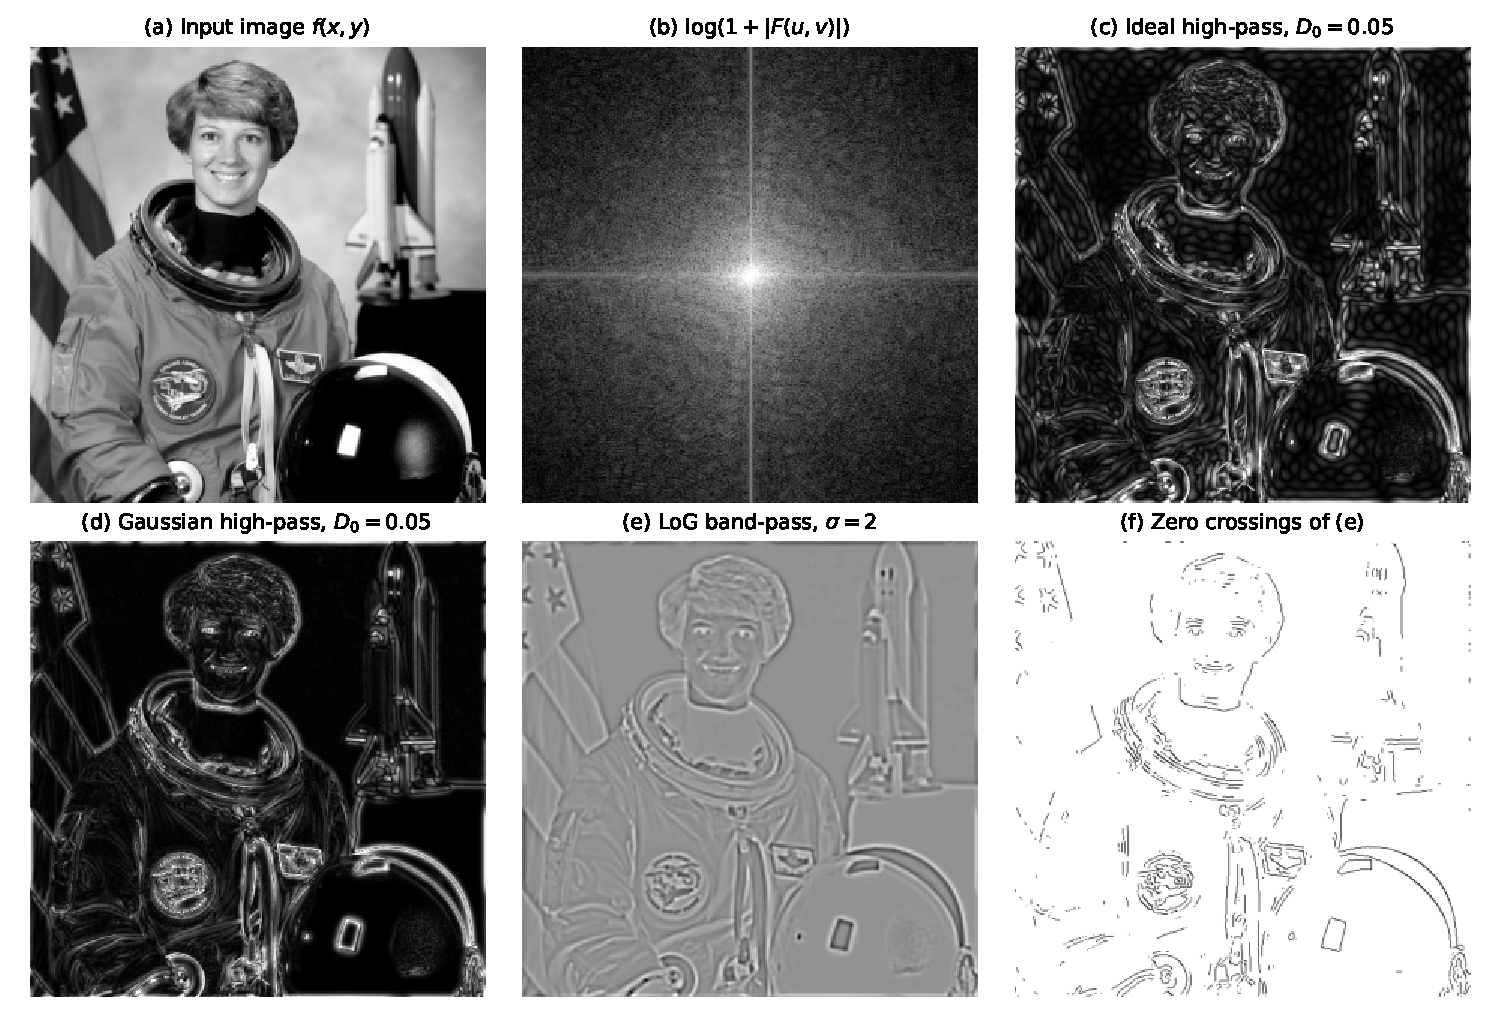
\includegraphics[width=0.7\textwidth]{fig_edges.pdf}
\caption{Frequency-domain edge detection on a $512\times512$ image, every filter applied as $G=HF$ followed by an inverse FFT. (b) Most energy sits near the origin; the bright cross comes from the image borders under the DFT's periodic assumption. (c,d) High-pass filters keep edges and discard smooth regions. (e,f) The LoG band-pass of Eq.~\eqref{eq:log} and its zero crossings trace edge contours.}
\label{fig:edges}
\end{figure}

\section{Frequency-domain filter design and the ringing problem}

A high-pass filter is one minus a low-pass: $H_{\text{HP}}=1-H_{\text{LP}}$, so $h_{\text{HP}}=\delta-h_{\text{LP}}$. With cutoff $D_0$ and $D=\rho$, three common choices are:
\begin{align*}
\text{Ideal:}&\quad H=\begin{cases}0,& D\le D_0\\ 1,& D>D_0\end{cases}\\
\text{Butterworth (order $n$):}&\quad H=\frac{1}{1+(D_0/D)^{2n}}\\
\text{Gaussian:}&\quad H=1-e^{-D^2/(2D_0^2)}
\end{align*}
\paragraph{Why the ideal filter rings.} The ideal low-pass is a disc of radius $D_0$ in frequency. Its inverse transform, computed in polar coordinates with the Bessel identity $\int_0^{2\pi}e^{j2\pi\rho r\cos\theta}d\theta=2\pi J_0(2\pi\rho r)$, is
\begin{equation}
h_{\text{LP}}(r)=\int_0^{D_0}2\pi\rho\,J_0(2\pi\rho r)\,d\rho=\frac{D_0\,J_1(2\pi D_0 r)}{r},
\end{equation}
a ``jinc'' with oscillating side lobes. Convolving an edge with it reproduces those oscillations as parallel ghost edges (the 2D Gibbs phenomenon). The Gaussian low-pass inverts to $2\pi D_0^2\,e^{-2\pi^2D_0^2r^2}$, which is positive everywhere with no side lobes, so the Gaussian high-pass produces no ringing. Figure~\ref{fig:ringing} shows the difference on a real image.

\subsection{Algorithm}
\begin{enumerate}[leftmargin=*,itemsep=2pt]
\item Pad the $M\times N$ image to $P\times Q=2M\times2N$. The DFT treats the image as periodic, and padding prevents wraparound, where the right edge convolves with the left.
\item Multiply by $(-1)^{x+y}$ to centre the spectrum, then compute $F(u,v)$ with the FFT in $O(PQ\log PQ)$.
\item Multiply by the chosen $H(u,v)$: $j2\pi u$ and $j2\pi v$ times $G_\sigma$ for a gradient, or $H_{\text{LoG}}$.
\item Inverse FFT, undo the $(-1)^{x+y}$, crop to $M\times N$.
\item Gradient route: threshold $|\nabla f|$, optionally with non-maximum suppression and hysteresis (Canny). LoG route: keep zero crossings whose slope exceeds a threshold.
\end{enumerate}
For large kernels, the FFT route costs $O(\log PQ)$ per pixel against $O(k^2)$ for direct convolution with a $k\times k$ kernel.



\begin{figure}[H]
\centering
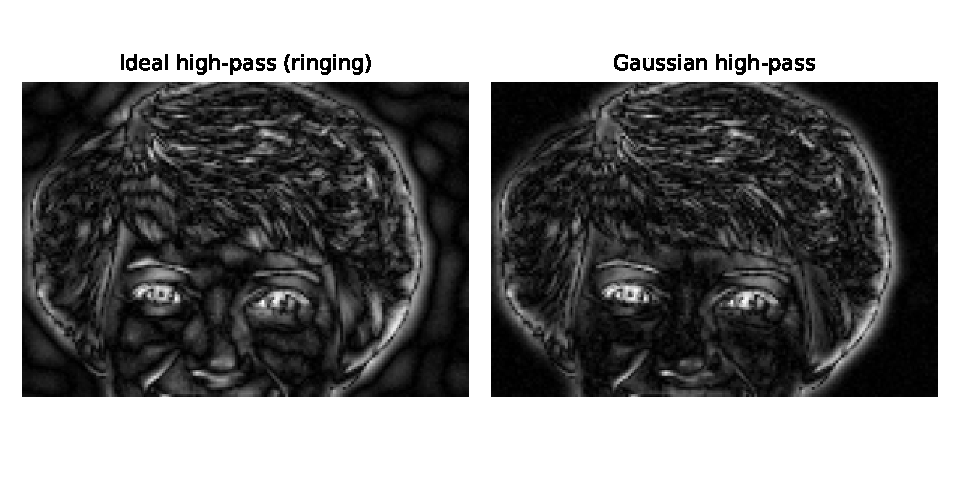
\includegraphics[width=0.5\textwidth]{fig_ringing.pdf}\\[2pt]
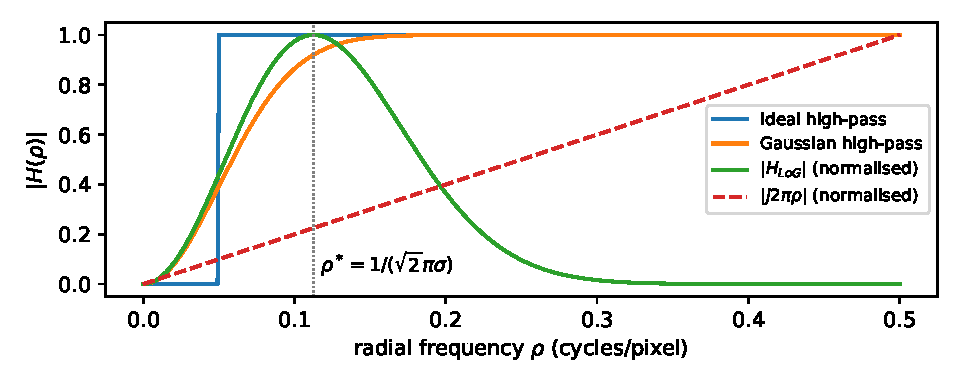
\includegraphics[width=0.56\textwidth]{fig_filters.pdf}
\caption{Top: zoom on the face. The ideal high-pass adds ripple bands parallel to each edge (the jinc side lobes); the Gaussian high-pass does not. Bottom: radial profiles $|H(\rho)|$. The pure derivative $|j2\pi\rho|$ keeps rising, so it amplifies noise; the LoG peaks at $\rho^*=1/(\sqrt2\pi\sigma)$ and returns to zero.}
\label{fig:ringing}\label{fig:filters}
\end{figure}

\section{Region segmentation in the frequency domain}

Edges and regions are two views of one spectrum. Inside a homogeneous region, intensity varies slowly and the local spectrum concentrates at low frequencies; at a boundary, the spectrum spreads out as in \eqref{eq:step}. Segmentation can therefore work from either side.

\subsection{Boundary route: close the edge map}
The LoG zero crossings form closed contours by construction, because the zero set of a smooth function separates positive from negative regions. Labelling the connected components of $\{\,g_{\text{LoG}}>0\,\}$ and $\{\,g_{\text{LoG}}<0\,\}$ gives a region segmentation directly.

\subsection{Region route 1: low-pass before thresholding}
Intensity thresholding (Otsu, as used in Questions 1 and 2) needs two well-separated histogram modes. Noise widens each mode by $\sigma_n$. A Gaussian low-pass shrinks the noise variance to
\[
\sigma_n^2\iint e^{-4\pi^2\sigma^2\rho^2}\,du\,dv=\frac{\sigma_n^2}{4\pi\sigma^2},
\]
so the modes narrow by a factor $2\sqrt{\pi}\,\sigma$ and the threshold separates regions more reliably. The price is a boundary blurred over roughly $\sigma$ pixels.

\subsection{Region route 2: texture segmentation with local spectra}
When two regions share the same mean brightness but differ in texture, the global spectrum mixes them. We need a spectrum localised around each pixel, the windowed (short-time) Fourier transform:
\begin{equation}
F_w(x,y;u,v)=\iint f(s,t)\,w(s-x,t-y)\,e^{-j2\pi(us+vt)}\,ds\,dt .
\end{equation}
With a Gaussian window, fixing one frequency $(u_0,v_0)$ turns this into a convolution with a \emph{Gabor filter}:
\begin{equation}
h_{u_0,v_0}(x,y)=e^{-\frac{x^2+y^2}{2\sigma^2}}\,e^{\,j2\pi(u_0x+v_0y)} .
\end{equation}
\paragraph{Transfer function of the Gabor filter.} By the modulation theorem, multiplying by $e^{j2\pi(u_0x+v_0y)}$ shifts the spectrum by $(u_0,v_0)$. Directly:
\[
H(u,v)=\iint e^{-\frac{x^2+y^2}{2\sigma^2}}\,e^{-j2\pi[(u-u_0)x+(v-v_0)y]}\,dx\,dy
=2\pi\sigma^2\,e^{-2\pi^2\sigma^2\left[(u-u_0)^2+(v-v_0)^2\right]} .
\]
The Gabor filter is a Gaussian band-pass centred on $(u_0,v_0)$: it selects one spatial frequency and one orientation, $\theta_0=\arctan(v_0/u_0)$.

\paragraph{Local energy features.} For a bank of $K$ filters, define
\begin{equation}
E_k(x,y)=\left(|h_k*f|^2\right)*g_{\sigma_E}(x,y),\qquad k=1,\dots,K .
\end{equation}
By Parseval's theorem, $|h_k*f|^2$ measures the energy the neighbourhood of $(x,y)$ carries in band $k$, and the extra Gaussian smoothing averages out the ripple of the carrier. Each pixel gets a feature vector $(E_1,\dots,E_K)$. A texture with a dominant frequency near $(u_k,v_k)$ produces a large $E_k$, so pixels are assigned to the region whose band dominates. For two textures $A$ and $B$ the rule is
\begin{equation}
\text{pixel}\in B \iff \log E_B(x,y)-\log E_A(x,y)>0,
\end{equation}
and the boundary is the zero level set of this log-ratio. The log makes the rule invariant to local contrast, because a contrast scale multiplies both energies by the same factor.

\paragraph{Resolution trade-off.} The window cannot be small in both domains. Measure spread as the standard deviation of $|h|^2$ in space and of $|H|^2$ in frequency. For the Gaussian envelope, $|h|^2\propto e^{-x^2/\sigma^2}$ gives $\Delta x=\sigma/\sqrt2$, and $|H|^2\propto e^{-4\pi^2\sigma^2u^2}$ gives $\Delta u=1/(2\sqrt2\,\pi\sigma)$, so
\begin{equation}
\Delta x\,\Delta u=\frac{1}{4\pi},
\end{equation}
the lower bound of the uncertainty principle. Gabor filters reach it exactly, which is why they are the standard choice. A large $\sigma$ separates textures with close frequencies but localises the boundary only to about $\sigma$ pixels; a small $\sigma$ locates the boundary sharply but confuses similar textures.

\begin{figure}[H]
\centering
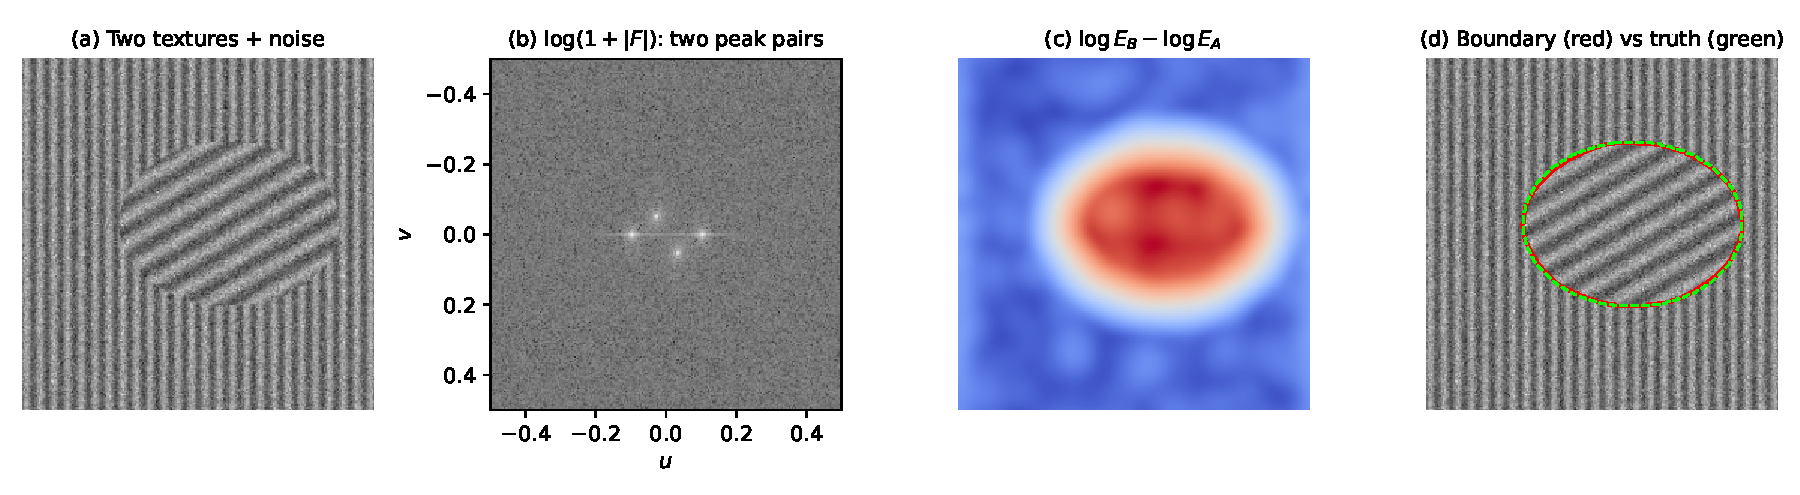
\includegraphics[width=\textwidth]{fig_texture.pdf}
\caption{Texture segmentation with Gabor energy. (a) An elliptical region of oblique stripes (0.06 cycles/px, $60^\circ$) inside vertical stripes (0.10 cycles/px), plus Gaussian noise with standard deviation 0.6 against a stripe amplitude of 1. (b) Each texture appears as a symmetric pair of spectral peaks. (c) Two Gabor band-passes, each built in the frequency domain as a pair of Gaussians at $\pm(u_0,v_0)$ with $\sigma=6$, give energies whose log-ratio separates the regions. (d) The zero level set (red) matches the true boundary (dashed green); 99.6\% of pixels are labelled correctly.}
\label{fig:texture}
\end{figure}

\subsection{Phase congruency: edges from the phase spectrum}
Magnitude-based detectors depend on contrast. The phase spectrum offers an alternative. Expand a 1D signal locally as $f(x)=\sum_n A_n\cos(n\omega x+\phi_n)$ and define
\begin{equation}
PC(x)=\frac{\left|\sum_n A_n\,e^{\,j(n\omega x+\phi_n)}\right|}{\sum_n A_n}\in[0,1].
\end{equation}
By the triangle inequality $PC=1$ exactly when every component has the same local phase. A step has the Fourier series $\frac{4}{\pi}\sum_k\frac{\sin((2k+1)\omega x)}{2k+1}$, and at $x=0$ every term sits at the same phase (a rising zero crossing), so $PC(0)=1$ at the edge. Scaling the contrast multiplies every $A_n$ by the same factor and leaves $PC$ unchanged, so phase congruency finds low-contrast boundaries that a gradient threshold misses.


\FloatBarrier
\section{Summary}

\begin{center}
\begin{tabular}{@{}lll@{}}
\toprule
Operation & Transfer function $H(u,v)$ & Role\\
\midrule
Gradient & $j2\pi u,\ j2\pi v$ & high-pass, edge strength and direction\\
Laplacian & $-4\pi^2\rho^2$ & isotropic high-pass, zero crossings at edges\\
Gaussian smoothing & $e^{-2\pi^2\sigma^2\rho^2}$ & low-pass, noise suppression\\
LoG & $-4\pi^2\rho^2e^{-2\pi^2\sigma^2\rho^2}$ & band-pass, peak at $\rho^*=1/(\sqrt2\pi\sigma)$\\
Gaussian high-pass & $1-e^{-\rho^2/(2D_0^2)}$ & edge enhancement without ringing\\
Gabor & $2\pi\sigma^2e^{-2\pi^2\sigma^2[(u-u_0)^2+(v-v_0)^2]}$ & frequency and orientation band-pass, texture\\
\bottomrule
\end{tabular}
\end{center}

Edges carry the high-frequency energy of an image, because the derivative theorem multiplies the spectrum by $j2\pi u$ and a step's spectrum decays only as $1/\rho$. Noise forces the detector to be a band-pass instead of a pure high-pass, and the LoG's parameter $\sigma$ picks the edge scale. For segmentation, low-pass filtering sharpens intensity histograms for thresholding, while local band energies from Gabor filters separate regions that differ in texture, with the uncertainty principle setting the trade-off between spectral discrimination and boundary accuracy.

\end{document}
